
% This LaTeX was auto-generated from MATLAB code.
% To make changes, update the MATLAB code and republish this document.

\documentclass{article}
\usepackage{graphicx}
\usepackage{color}

\sloppy
\definecolor{lightgray}{gray}{0.5}
\setlength{\parindent}{0pt}

\begin{document}

    
    
\subsection*{Contents}

\begin{itemize}
\setlength{\itemsep}{-1ex}
   \item clear workspace variables
   \item Make a vector and plot
   \item Create math in MATLAB publishing
   \item Make bullets
   \item How about a numbered list? Just use \# instead of *
   \item You can do hyperlinks as well
   \item Types of text
\end{itemize}
\begin{verbatim}
% Author: Dylan Mikesell
% Created: 20 September 2016
% Last modified: 21 September 2016
\end{verbatim}


\subsection*{clear workspace variables}

\begin{verbatim}
clear all;
close all;
\end{verbatim}


\subsection*{Make a vector and plot}

\begin{verbatim}
x = linspace(0,2*pi,180/pi);
y = sin(x);

h = figure;
plot(x,y,'k');
\end{verbatim}

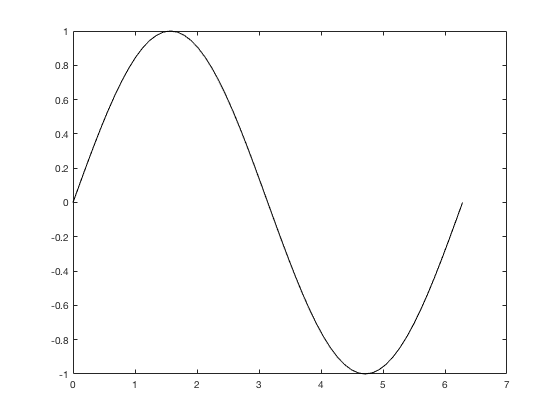
\includegraphics [width=4in]{MatlablPublishingExample_01.png}


\subsection*{Create math in MATLAB publishing}

\begin{par}
This is called inline math with a single dollar sign (\$) around the math.
\end{par} \vspace{1em}
\begin{par}
$y = \sin(x)$
\end{par} \vspace{1em}
\begin{par}
This is called display math with two dollar signs (\$\$) around the math.
\end{par} \vspace{1em}
\begin{par}
$$y = \sin(x)$$
\end{par} \vspace{1em}


\subsection*{Make bullets}

\begin{itemize}
\setlength{\itemsep}{-1ex}
   \item This is the first bullet
   \item This is the second bullet
\end{itemize}
\begin{verbatim}
% The trick is the '% *' symbols. Also, make sure there are no empty lines
% betweeen the bullets and the '%% section title' line. Otherwise, the
% bullets are not interpreted as bullets. If you have blank lines, make
% sure to comment those lines. Same goes for the math examples above.
\end{verbatim}


\subsection*{How about a numbered list? Just use \# instead of *}

\begin{enumerate}
\setlength{\itemsep}{-1ex}
   \item ITEM1
   \item ITEM2
\end{enumerate}


\subsection*{You can do hyperlinks as well}

\begin{par}
\begin{verbatim}GEOS397\end{verbatim}
\end{par} \vspace{1em}
\begin{verbatim}
% Note the space in between the URL and the text that will be linked.
\end{verbatim}


\subsection*{Types of text}

\begin{par}
\textbf{You can write in bold.}
\end{par} \vspace{1em}
\begin{par}
\textit{You can write in italic.}
\end{par} \vspace{1em}
\begin{verbatim}
% Note the *a* notation for bold and _a_ for italic.
\end{verbatim}



\end{document}
    
